%%%%%%%%%%%%%%%%%%%%%%%%%%%%%%%%%%%%%%%%%%%%%%%%%%%%%%%%%%%%%%%%%%%%
%% I, the copyright holder of this work, release this work into the
%% public domain. This applies worldwide. In some countries this may
%% not be legally possible; if so: I grant anyone the right to use
%% this work for any purpose, without any conditions, unless such
%% conditions are required by law.
%%%%%%%%%%%%%%%%%%%%%%%%%%%%%%%%%%%%%%%%%%%%%%%%%%%%%%%%%%%%%%%%%%%%

\documentclass[
  color, %% This option enables colorful typesetting. Replace with
         %% `monochrome`, if you are going to print the thesis on
         %% a monochromatic printer.
  table, %% Causes the coloring of tables. Replace with `notable`
         %% to restore plain tables.
  lof,   %% Prints the List of Figures. Replace with `nolof` to
         %% hide the List of Figures.
  lot,   %% Prints the List of Tables. Replace with `nolot` to
         %% hide the List of Tables.
  %% More options are listed in the class documentation at
  %% <http://mirrors.ctan.org/macros/latex/contrib/fithesis/fithesis/guide/mu/fi.pdf>.
]{fithesis3}
%% The following section sets up the locales used in the thesis.
\usepackage[resetfonts]{cmap} %% We need to load the T2A font encoding
\usepackage[T1,T2A]{fontenc}  %% to use the Cyrillic fonts with Russian texts.

\usepackage[
  main=english, %% By using `czech` or `slovak` as the main locale
                %% instead of `english`, you can typeset the thesis
                %% in either Czech or Slovak, respectively.
  german, russian, czech, slovak %% The additional keys allow
]{babel}        %% foreign texts to be typeset as follows:
%%
%%   \begin{otherlanguage}{german}  ... \end{otherlanguage}
%%   \begin{otherlanguage}{russian} ... \end{otherlanguage}
%%   \begin{otherlanguage}{czech}   ... \end{otherlanguage}
%%   \begin{otherlanguage}{slovak}  ... \end{otherlanguage}
%%
%% For non-Latin scripts, it may be necessary to load additional
%% fonts:
\usepackage{paratype}
\def\textrussian#1{{\usefont{T2A}{PTSerif-TLF}{m}{rm}#1}}
\usepackage{xcolor} 
\newcommand{\todo}[1]{\textcolor{red}{\textbf{#1}}}
\usepackage{listings}
\usepackage[binary-units=true]{siunitx}
%%
%% The following section sets up the metadata of the thesis.
\thesissetup{
    university    = mu,
    faculty       = fi,
    type          = bc,
    author        = Samuel Petrovič,
    gender        = m,
    advisor       = Adam Rambousek,
    title         = {The effects of age on file system performance},
    TeXtitle      = {The effects of age on file system performance},
    keywords      = {filesystem, xfs, IO operation, aging, fragmentation ...},
    TeXkeywords   = {filesystem, xfs, IO operation, aging, fragmentation ...},
}
\thesislong{abstract}{
    This is the abstract of my thesis, which can

    span multiple paragraphs.
}
\thesislong{thanks}{
    This is the acknowledgement for my thesis, which can

    span multiple paragraphs.
}
%% The following section sets up the bibliography.

\usepackage{csquotes}
\usepackage[              %% When typesetting the bibliography, the
  backend=bibtex,          %% `numeric` style will be used for the
  style=numeric,          %% entries and the `numeric-comp` style
  citestyle=numeric-comp, %% for the references to the entries. The
  sorting=none,           %% entries will be sorted in cite order.
  sortlocale=auto         %% For more unformation about the available
]{biblatex}               %% `style`s and `citestyles`, see:
%% <http://mirrors.ctan.org/macros/latex/contrib/biblatex/doc/biblatex.pdf>.
\addbibresource{citations2.bib} %% The bibliograpic database within

                          %% the file `example.bib` will be used.
\usepackage{makeidx}      %% The `makeidx` package contains
\makeindex                %% helper commands for index typesetting.
%% These additional packages are used within the document:
\usepackage{paralist}
\usepackage{amsmath}
\usepackage{amsthm}
\usepackage{amsfonts}
\usepackage{url}
\usepackage{menukeys}
\usepackage{pdfpages}
\usepackage{mwe}
\usepackage{cleveref}

\renewcommand{\lstlistingname}{Example}
\renewcommand{\lstlistlistingname}{List of \lstlistingname s}


\begin{document}
\chapter{Introduction}
File systems remain an important part of modern storage solutions.  Large, growing databases, multi-media and other storage based applications need to be supported by high-performing infrastructure layer of storing and retrieving information. Such infrastructure have to be provided by operating systems (OS) in form of file system.

Originally, file system was a simple tool developed to handle communication between OS and physical device, but today, it is a very complex piece of software with large set of tools and features to go~with.

Performance testing is an integral part of development cycle of most of produced software. Because of growing complexity of file systems, performance testing took of as an important part of file system evaluation.

The standard workflow of performance testing is called out-of-box testing. Its principle is to run benchmark (i.e. testing tool) on a clean instance of OS and on a clean instance of tested file system~\cite{Traeger:2008:NYS:1367829.1367831}. Generally, this workflow present stable and meaningful results, yet, it only gives overall idea of file system behavior in early stage of its life cycle. 

File systems, as well as other complex software is subjected to progressive degradation, referred to as software aging~\cite{Cotroneo:2014:SSA:2543749.2539117}. Causes of file system aging are many, but mostly fragmentation of free space, unclustered blocks of data and unreleased memory. This degradation cause problems in performance and functionality over time. Understanding of performance changes of aged file system can help developers to implement various preventions of aging related problems. Furthermore, aging testing can help developers with implementation of long-term performance affecting features.

Researching of file system aging can by done in two stages, aging the file system and testing of the aged instance. In the first stage, observation about \emph{evolution} of fragmentation and performance can be made. The second stage brings insight into \emph{state} of performance of aged file system.

In the first part, this thesis describe implementation of two flexible tests, which correspond with afformentioned stages.
 
In the first-stage testing, file system is aged using open-source benchmark fs-drift. While aging the file system, fragmentation of free space and latency of IO operations is periodically recorded. After the aging process, additional information about file fragmentation and file size distribution is recorded as well. Once this information is gathered, image of aged file system instance is created. To save space, only metadata of created file system is used, since content of created files is random and therefore irrelevant.

Created images are then used in second-stage testing. By using created images, higher stability and consistency of results is achieved. By reloading the file system image on the device, it is possible to bring the file system to the original aged state, therefore for every performance test, the same file system layout is available.

In the second-stage testing, file system is brought to the aged state by reloading image corresponding with desired testing configuration. Before every performance test, some volume is released from file system, so the performance test has space to test on. By using this workflow, it may be possible to simulate behavior of aged file systems at different stages of volume usage.

%The aging tests implemented in this thesis are established as part of testing cycle in Red Hat Kernel Performance team.

In the later parts of this thesis, usage of developed tests on different configurations of file systems and storage is demonstrated. The subject of research are differences between popular Linux file systems (XFS, Ext4) and storage technology (solid state and hard disk drives) in context of aging. Because of nature of collected data, a processing tool was implemented to parse large amount of information into human readable reports. All the generated reports are part of this thesis in form of Appendix A.

In the second chapter, the text present already conducted research of effects of age and fragmentation on file system performance. Third chapter describes used file systems and theirs main features. Chapter 4 introduce tools used in implementation of tests while describing their relevant features. Chapters 5 and 6 describe actual implementation of mentioned tests. Chapter 7 describes testing environment and presents used storage technology. Chapter 8 presents the results obtained by using created tests. The research is focused describing the effect of aging file systems, differences between file systems in terms of aging and relations of underlying storage to performance of aged file system. In the conclusion chapter, I discuss the effects of age on file system performance as well as recommendations for this type of testing. Furthermore, future of testing of file system performance and aging is discussed.

Appendix A contains complete reports generated from conducted tests. Appendix B contains examples of usage of used tools.  

\chapter{Related work}
In this chapter I present different approaches of file system aging and fragmentation research described and implemented in the past. The first section discuss usage of collected data to create aging workload. The second section discuss possibilities of aging the file system artificially, without pre-collected data.

\section{Aging file system using real-life data}
This approach is based on modeling the aged file system using data collected from file systems used in real-life environment.

Such data can be in form of snapshots (i.e. images) of file systems, as was thoroughly described by Smith and Seltzer~\cite{Smith:1997:FSA:258623.258689}.

The snapshots were collected nightly over a long period of time (one to three years) on more then fifty file systems. By comparing pairs of snapshots in the sequence, performed operations were estimated, resulting in a very realistic aging workload. However, as some studies suggest, most of files have life span shorter than 24 hours~\cite{Ousterhout:1985:TAU:323647.323631}. Therefore, as Smith and Seltzer admit, by snapshoting every night, this process does not account for most of the created files, resulting in loss of important part of data.

Furthermore, to age a file system sized $\SI{1024}{\mega\byte}$, $\SI{87.3}{\giga\byte}$ of data had to be written, taking 39 hours to complete, rendering the workflow impractical for in-production testing needs.

Smith and Seltzer also defined a layout score as a method to evaluate fragmentation of a file system. Layout score is defined as a fraction of blocks of file, which are contiguously allocated. Files of one block size are ignored, since they can't be fragmented, and for every file, first block is ignored too. Evaluation of the whole file system is then computed as an aggregated layout score of all files.

The problem resulting from not tracking shortly lived files can be solved by another approach called collecting traces. Traces are sequences of IO operations performed by OS, captured at various levels (system call, drivers, network, etc.). The sequence of operations can be replayed back to the file system, aging it in a realistic manner.

Overall, using real-life data to age file systems brings realistic results, but at a cost of higher expenses, such as storing the collected data. Additionally, to cover cases of different types of file system usage, data from several such file systems have to be collected, expanding the amount of needed data even further. Such materials are not always available, rendering this type of approach useful only in cases the researcher is already in their possession.

\section{Synthetic aging simulation}
Synthetic aging is a type of aging that does not require real-life data for its running. It relies on purely artificial workload performed on a file system, invoking aging factors, such as fragmentation.

Fast file system aging was described as a part of a trace replay benchmark called TBBT~\cite{Zhu:2005:TSA:1251028.1251052}. This type of aging consists of sequence of interleaving append operations on a set of files. By controlling the amount of files involved in the process, researchers had great control over fragmentation. Such workflow, while creating desired fragmentation, is however quite unrealistic, making the results of testing on such file system questionable~\cite{Traeger:2008:NYS:1367829.1367831}.

Another attempt of inducing fragmenetation was made in an empirical study of file system fragmentation in mobile storage systems~\cite{ji2016empirical}. The aging process consisted of filling the device by alternative creation of files larger or equal to $\SI{100}{\mega\byte}$ and smaller or equal $\SI{100}{\kilo\byte}$. After 100\% file system utilization was reached, 5\% of files was randomly deleted. 

However, for truly realistic insight, a workflow generator which tries to mimic real-life usage can more suitable.

A workload generator such as fs-drift~\cite{fs-drift:github}, can be used (while carefully configured) to simulate desired long term real-life usage. While running, fs-drift is creating requests of variety of IO operations. The probability with which would be operation chosen can be controled by workload table. In addition, this tool offers different probability distributions of file access, making it easier to mimic behavior of natural user. Furthermore, whole process is highly configurable, making it possible to simulate various types of file system usage. Such qualities predispose fs-drift to be capable of conduction of more realistic results than mentioned attempts.

\chapter{File system and storage devices}
In this chapter, I present basic information about used file systems and storage devices and its features relevant to performance and aging.

\section{File systems}
File system is a set of tools, methods, logic and structure to control how to store and retreive data on and from device.

The system stores files either continuously or scattered across device. The basic accessed data unit is called a block, which capacity can be set to various sizes. Blocks are labeled as either free or used.

Files which are non-contigous are stored in form of extents, which is one or more blocks associated with the file, but stored elsewhere.  

Information about how many blocks does a file occupy, as well as other information like date of creation, date of last access or access permissions is known as metadata, e.g. data about stored data. This information is stored separately from the content of files. On modern file systems, metadata are stored in objects called index nodes (e.g. inodes). Each file a file system manages is associated with an inode and every inode has its number in an inode table. On top of that the file system stores metadata about itself (unrelated to any specific file), such as information about bad sectors, free space or block availability in a structure called superblock.

In this thesis, targeted file systems are two most popular Linux file systems~\cite{Lu:2013:SLF:2591272.2591276}, XFS~\cite{xfs:qhe} and Ext4~\cite{ext4:qhe}, which are also main Red Hat supported file systems. These file systems belong to the group of file systems called journaling file systems.

Journaling file system keeps a structure called journal, which is a buffer of changes not yet commited to the file system. After system failure, these planned changes can be easily read from the journal, thus making the file system easily fully operational, and in correct and consistent state again.

\subsection{XFS}
XFS is a 64-bit journaling file system known for its high scalability (up to $\SI{9}{\exa\byte}$) and great performance. Such performance is reached by architecture based on allocation groups.

Allocation groups are euqally sized linear regions within file system. Each allocation group manages its own inodes and free space, therefore increasing parallelism. Architecture of this design enables for significant scalability of bandwidth, threading, and size of file system, as well as files, simply because multiple processes and threads can access the file system simultaneously.

XFS allocates space as extents stored in pairs of $B^+$ trees, each pair for each allocation group (improving performance especially when handling large files). $B^+$ trees is indexed by the length of the free extents, while the other is indexed by the starting block of the free extents. This dual indexing scheme allows efficient location of free extents for IO operations.

Prevention of file system fragmentation consist mainly of a features called delayed allocation and online defragmentation.

Delayed allocation, also called allocate-on-flush is a feature that, when a file is written to the buffer cache, substracts space from the free space counter, but won't allocate the free-space bitmap. The data is held in memory until it have to be stored because of system call. This approach improves the chance the file will be written in a contiguous group of blocks, avoiding fragmentation and reducing CPU usage as well.

\subsection{Ext4}
Ext4, also called fourth extended filesystem is a 48-bit journaling file system developed as successor of Ext3 for Linux kernel, improving reliability and performance features. Ext4 is scalable up to $\SI{1}{\exbi\byte}$ (approx. $\SI{1.15}{\exa\byte}$). Traditional Ext2 and Ext3 block mapping scheme was replaced by extent based approach similar to XFS, which positively affects performance.

Similarly to XFS, Ext4 use delayed allocation to increase performance and reduce fragmentation. For cases of fragmentation that still occur, Ext4 provide \texttt{e4defrag} tool to defragment either single file, or whole file system. Performance penalties were, however, recognized and online defragmentation workflow was proposed by Sato~\cite{sato2007:ext4}.


%Ext4 provide support for online defragmentation~\cite{sato2007:ext4} and \textit{e4defrag} tool to defragment either single file, or whole file system.


\section{Storage}
\subsection{Hard disk drive}
A hard-disk drive (i.e. HDD) is a type of storage device which use one or more magnetic plates to store data. Data can be retreived by rotating the plates and positioning magnetic read-write heads. The plates rotate at stable speed at around 7500\,rpm (and more on enterprise-level hardware).

Since the parts of HDD have to physically move to reach desired location, there is a latency to the data access. The time for magnetic head to find next relevant block of data is called a \emph{seek time}. Because the length of seek time has significant impact on overall IO performance, OS have to do a lot of optimising, such as pre-fetching.

Obviously, block layout would have a large impact on performence of this kind of device. The amount of fragmentation (thus aging) affect the number of performed seeks. This cause the pressure on file system to store data more contiguously and also cluster related data.

\subsection{Solid state drive}
Solid state drive (i.e. SSD) is  a type of storage device which use integrated cirquit to store and retreive data. SSD has no moving parts, therefore the data access is purely electronic, which results in lower access time and latency than HDD.

However, on SSDs, data cannot be directly overwritten (as in HDDs). The cell of an SSD can only be directly written to, therefore have to be erased before writing. Moreover, due to physical construction limits, write operation can be conducted to one page (4-$\SI{16}{\kilo\byte}$), but erasure have to be done to a whole block (128 to 512 pages). Therefore, if OS have to rewrite some blocks (e.g. update metadata), the data have to be read, erased from the drive and written back modified. This effect, known as write amplification, can have significant impact on performance of file systems. 

In addition, the memory cell can be rewritten finite amount of times, therefore, a form of wear leveling has to be employed. Wear leveling prevents frequently accessed blocks from exhaustion of cells life-cycle by moving files around the device.

Static wear leveling rotates even unused files around the drive to ensure equal wear. However, deleting file in file system doesn't always ensure its deletion on the device. Typically, the file is only marked as deleted, but this information is not submited to underlying device itself. However, files that are not valid for file system anymore can still circulate on the device, increasing its wear and write amplification, since there are less free block that could have been.

To decrease this effect, trim commands were introduced. Trim command communicate to SSD all the deletions that were realised in the file system, so the drive can erase blocks accordingly. Nevertheless this operation is reducing performance of IO operations while being conducted, it can increase overall performance and life time of an SSD.



\chapter{Environment setup and benchmark tools}
In this chapter, I present tools which were used to implement automated tests for creating and storing aged file systems and measuring their performance. Furthermore, I describe the main features and means of their usage. All the presented tools are open source projects.

\section{Beaker}
Beaker is an open source project aimed at automating testing workflow. The software can provision system from a pool of labs, install OS and packages, configure environment and perform tasks. The whole process is guided by sequence of instructions in an XML format. Examples can be found in Apendix A.

The workflows created as a part of this thesis are implemented in form of Beaker task packages, which can be directly used by Beaker. A task package has to include Makefile which can then run other scripts included in the package. Scripts can also communicate with Beaker via API installed on every machine.  By this means, tests can send logs or report their status on server while running.

\section{Storage generator}
Storage generator is a Beaker task developed by Jozef Mikovič. It is capable of automated configuration of storage on a machine. In a single-device mode, storage generator simply creates new partition on a given device and creates and mounts file system. In a recipe mode, storage generator follows set of bash instruction to create more advanced configurations such as merging multiple devices using LVM, creating LVM cache or encrypted volume.

The creation of XFS file system is standard, but Ext4 file system is created with additional option, disabling \emph{lazy init}. Lazy init is a feature which allows for fast creation of file system by not allocating all the available space at once. The space is allocated later, as the file system grows. Such additional allocation, however would skew data collected in the first hours of the test, therefore it is disabled in these tests.

\section{FIO}
Flexible Input/Output tool is a workload generator written by Jens Axboe. It is a tool well known for it's flexibility as well as large group of users and contributors. The flexibility is integral for conductuing less artifical and more natural performance tests. However, approaching more natural test behavior, stability of results drop, so ideal equilibrium between these two requirement has to be found.

FIO accepts the workload specification as either a configuration file or a single line. Multiple different jobs can be specified as well as global options valid for every job. 

There is a possibility to choose from 4 IO operations to be performed (or their mix). These operations are sequential write, sequential read, random write and random read. Verification of the issued data is offered as well. Size of generated file and block size can be controlled too and it can be either stable or chosen from given range. For cache-tiering workloads, different random distributions (e.g. Zipf) can be specified. FIO also supports process forking and threading.

After the test, FIO generates overall report of measured performance. However, logging of multiple properties can be enabled, giving researchers even more oversight about the nature of file system performance.

\section{Fs-drift}
Fs-drift is a very flexible aging test, which can be used to simulate lots of different workloads. The test is based on random file access and randomly generated mix of requests. These requests can be writes, reads, creates, appends, truncates or deletes.

At the beginning of run time, the top directory is empty, therefore \texttt{create} requests success the most, other requests, such as \texttt{read} or \texttt{delete}, will fail because not many files has yet been created. Over time, as the file system grows, \texttt{create} requests began to fail and other requests will more likely succeede. File system will eventually reach a state of equilibrium, when requests are equaly likely to execute. From this point, the file system would not grow anymore, and the test runs unless one of the stop conditions are met.

The mix of operation probabilities can be specified in separate csv file. Fs-drift will try to issue more \texttt{create} operations at the beggining of testing, so other operations execute with higher likeliness.

The file to perform a request on is randomly chosen from the list of indexes. If the type of random distribution is set to \emph{uniform}, all indexes have the same probability to be chosen, see \ref{fig:rand1}. However, if the type of random distribution is set to \emph{gaussian}, the probability will behave according to normal distribution with the center at index 0 and width controled by parameter \texttt{gaussian-stddev}. This is usefull for performing cache-tiering tests. Please note, that file index is computed as modulo maximal number of files, therefore instead of accessing negative index values, the test access indexes from the other side of spectrum, see Figure \ref{fig:rand2}

Furthermore, fs-drift offers one more option to influence random distribution. After setting parameter \texttt{mean-velocity}, fs-drift will choose files by means of moving random distribution. The principle relies on a simulated time, which runs inside the test. For every tick of the simulated time, the center of bell curve will move on the file index array by the value specified by \texttt{mean-velocity} parameter. By enabling this feature, the process of testing moves closer to reality by simulating more natural patterns of file system access (the user won't access file system randomly, but rather works with some set of data at a time). On Figure \ref{fig:rand3}, you can see bell curve moving by 5 units two times.

\begin{figure}[!htb]
    \centering
    \begin{minipage}{\textwidth}
        \centering
        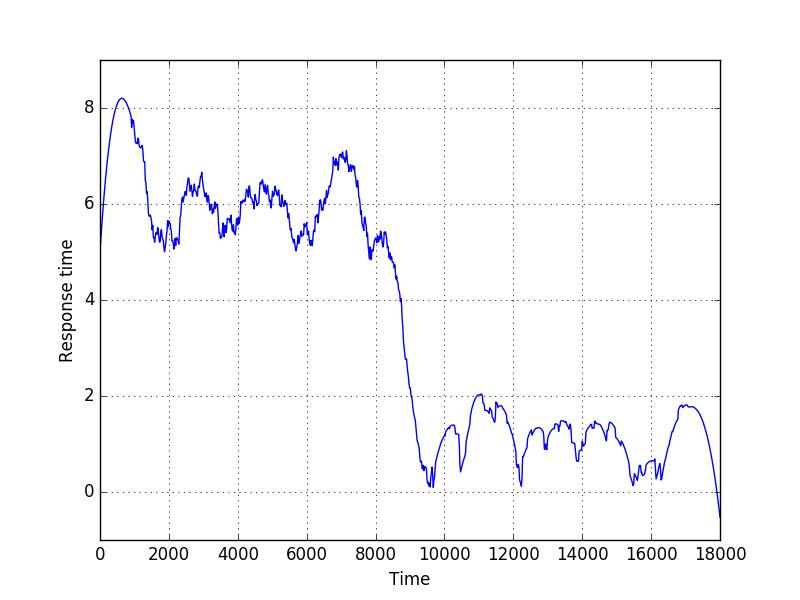
\includegraphics[width=0.7\textwidth]{../scripts/fig1.png}
        \caption{Uniform distribution of file access}
\label{fig:rand1}
    \end{minipage}\hfill
    \begin{minipage}{\textwidth}
        \centering
        \includegraphics[width=0.7\textwidth]{../scripts/fig2.png}
        \caption{Normal distribution of file access}

\label{fig:rand2}
    \end{minipage}

\end{figure}
\begin{figure}
    \begin{minipage}{\textwidth}
        \centering
        \includegraphics[width=0.7\textwidth]{../scripts/fig3.png}
        \caption{Moving random distribution}
\label{fig:rand3}
    \end{minipage}
\end{figure}

%For purpose of this thesis, several changes had to be made to the original code. Besides small errors like invalid Readme information, a bug in code had to be repaired, otherwise the fs-drift would not delete files while issuing \textit{delete} operation, marginally affecting aging process. Without this fix, the volume would just saturate and remain in more or less consistent state for the rest of the runtime.

%Additionally, to be able to inspect and work with the file system while aging process is still running, I added an option to specify \textit{pause file}. If the pause file is present, the fs-drift would not issue any requests and waits until the file is removed\footnotemark[1].
%\footnotetext[1]{For all the changes made to master branch of fs-drift, see ...}

Fs-drift offers even more parameters to control the test run such as number of directories, levels of directories, or enabling \texttt{fsync}/\texttt{fdatasync} to be called. To stop the fs-drift, one of the stop conditions have to be met. The stop condition can be either reached maximal number of performed operations, running out of time, or apparance of stop file.

For evaulation of the aging process, fs-drift can log latency of the performed opperations. However, the log doesn't differentiate between the operations, which could be usefull for further research.

Used configuration of fs-drift for purposes of aging testing is further described in Chapter~\ref{text:aging}.

\subsection{Changes to original code}
\label{text:fsdrift_changes}
Several changes had to be made to the original code prior to testing.

The most obvious problem with the tools was, that it did not conduct \texttt{delete} operations. As stated, deleting files is quite crucial to file system aging.

Another problem emerged when gathering statistics of response time evolution through the aging process. Since the tool is generating the IO requests at random, sometimes error occurs. Most operations need the file to exist to success, but sometimes, the file is non-existent. The problem with response time logging was, it logged the response time even if the operation didn't carry, causing noise in the data.

Further problem with response time logging was, it didn't differentiate between operations. Such distinction could greatly affect the way researchers can find problems with file system evolution.

As mentioned, possibility of specifying \emph{pause file} was added, making the fs-drift easy to pause for file system contents inspection.

Another feature added to fs-drift was non-uniform distribution of file sizes. Originally, fs-drift only uniform distribution to choose file size from zero to specified maximum size. Such implementation offers very little control over file size distribution and is quite unrealistic. Therefore, possibility to request natural file size distribution was added. As a reference for file size distribution, five year old study of file system metadata was used~\cite{agrawal2007five}. Figure 3 shows measured file size distribution of used file systems. To mimic this layout, log-normal distribution was modeled. The shape of resulting distribution is shown in Figure~\ref{fig:lognormal}.

The version used for testing in this thesis have all afformentioned features implemented and problems repaired. The code is also included in eletronic appendix.

\begin{figure}[!htb]
    \begin{minipage}{\textwidth}
        \centering
        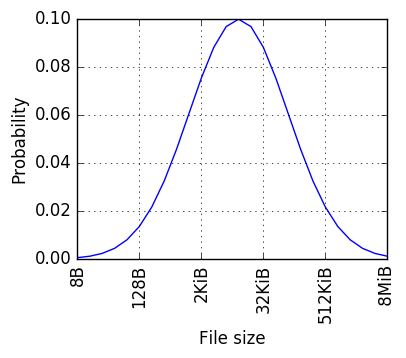
\includegraphics[width=0.7\textwidth]{../scripts/dist3.png}
        \caption{Logarhitmic normal distribution of file size}
\label{fig:lognormal}
    \end{minipage}
\end{figure}












\chapter{Aging the file system}\label{text:aging}
In this chapter, I describe process of developement of file system aging workflow and its implementation as a form of automated test.

\section{Aging process}
As mentioned, fs-drift was used as a mean of aging the fresh file system, bringing it to the aged, fragmented state. Fs-drift is quite flexible, therefore a lot of parameters and their impact on the final layout had to be considered.

First, the amount of fullness had to be taken into account. Heavily used file systems tend to be full at amounts ranging from 65 to 100 percent~\cite{agrawal2007five}. However, fs-drift does not offer an option to directly control the fullness of the file system. As the creator states in README, to fill a file system, maximum number of files and mean size of file should be defined such that the product is greater than the available space. Parameters to overload the volume are not difficult to come up with. The problem is, the random nature of the test doesn't allow for meaningfull reporoducibility of the reached equilibrium. In most cases, fs-drift plainly saturates given volume, so utilization remains at 100\% through the rest of the testing time. This drawback was overridden by a change in fs-drift code\footnotemark[1]. By adding the possibility to pause fs-drift, other processes can stop fs-drift to generate IO requests if the file system usage reaches a specified amount and release some space. This way, desired amount of maximal utilization can be reached.

\footnotetext[1]{For all the changes made to original code of fs-drift, see Subsection \ref{text:fsdrift_changes}}

Duration of the test is an important factor as well. In general, the testing time should be long enough for the environment to stabilise. After developing a test, it is necessary to conduct few pilot runs to confirm if any stabilisation of performance occur and set the duration accordingly for best effectivity

% When considering file system aging, 


%the test should spend most of the run time after the saturation phase (e.g. the phase of filling the file system to a desired fullness). 



%. On the other hand, for the test to be usefull in professional environment, testing time should not be too long. The goal is to maximize testing correctness while minimising the time for the test to complete. The ideal duration of testing is discussed and experimented with in Section~\ref{text:duration}

Fs-drift offers to control testing length by elapsed time. The elapsed time is computed as current time substracted from starting time. However, pausing the fs-drift to release space, examine file system, etc. resulted in non-uniform testing time across runs. Therefore, testing length by operation count is used in conducted tests.

File size is another important factor of succesfull simulation. To consider a simulation succesfull, resulting layout should have similar file size distribution as real-life file systems. For that reasons, when testing, natural file size distribution is turned on. The specifics of natural file distribution are described in Subsection~\ref{text:fsdrift_changes}.

During the test, all available file operations are used, with more weight placed on layout alterning operations (create, delete, truncate, append, random write). The non-alterning operations are there to verify, if any performance drop occur during the aging process.

\section{File system images}
File system images can be created by using tools developed to inspect file systems in case of emergency. For Ext* file systems, there is a tool called \texttt{e2image} and for XFS, \texttt{xfs\_metadump}. Both tools create images as sparse files, so compression is needed.

\texttt{E2image tool} can save whole contents of a file system or just its metadata and offers compresion of image as well. Created images can be further compressed by tools such \texttt{bzip2} or \texttt{tar}. Such images can be later reloaded back on a device. From that point, file system can be mounted. Example~\ref{ex:e2image1} shows creating file system image using \texttt{e2image} tool. Example~\ref{ex:e2image2} shows reloading image on device.

\lstset{language=bash, 
numbers=none, 
frame=single, 
commentstyle=\color{dkgreen}, 
basicstyle={\scriptsize\ttfamily}, 
keywordstyle=\color{blue}, 
%identifierstyle=\color{blue}, 
stringstyle=\color{red},
captionpos=t,
showstringspaces=false,
breaklines=true,
breakatwhitespace=false,
tabsize=3,
caption={sdad},
}

\begin{lstlisting}[language=bash, label={ex:e2image1}, caption={Creating compressed image using \texttt{e2image}}][frame=single]
  $ e2image -Q $DEVICE $NAME.qcow2
\end{lstlisting}

\begin{lstlisting}[language=bash, label={ex:e2image2}, caption={Reloading compressed image}][frame=single]
  $ e2image -r $NAME.qcow2 $DEVICE
\end{lstlisting}

\texttt{Xfs\_metadump} saves XFS file system metadata to a file. Due to privacy reasons file names are obsfucated (this can be disabled by -o parameter). As well as \texttt{e2image} tool, the image file is sparse, but \texttt{xfs\_metadump} doesn't offer a way to compress the output. However, output can be redirected to stdout and compressed further on. Generated images, when uncompressed, can be reloaded back on device by tool \texttt{xfs\_mdrestore}. File system can be then mounted and inspected as needed. Example~\ref{ex:xfs_metadump} shows creating file system image using \texttt{xfs\_metadump}. Example~\ref{ex:xfs_mdrestore} shows reloading image on device using \texttt{xfs\_mdrestore}.

\begin{lstlisting}[language=bash, label={ex:xfs_metadump}, caption={Creating compressed image using \texttt{xfs\_metadump}}][frame=single]
  $ xfs_metadump -o $DEVICE -|bzip2 > $NAME
\end{lstlisting}

\begin{lstlisting}[language=bash, label={ex:xfs_mdrestore},caption={Reloading image using \texttt{xfs\_mdrestore}}][frame=single]
  $ xfs_mdrestore $NAME $DEVICE
\end{lstlisting}

\section{Implementation details}
Workflow of image creating is contained in the Beaker task drift\_job. After extracting fs-drift, the main script starts python script, which handles the process of running fs-drift. Settings of fs-drift are passed as a parameter and then parsed inside the script.

Before running the fs-drift, asynchronous thread \texttt{async\_worker} is triggered. \texttt{Async\_worker} offers ways to additionally control testing and to work with file system while the test is running. The thread wakes up at specified intervals. Upon awakening, fs-drift is paused, then free space fragmententation and file system usage is logged. If the usage reaches defined limit, specified amount of space is randomly released from file system. If the test runs on an SSD, \texttt{fstrim} can be optionally called. Furhtermore, when all mentioned operations are done, the thread calls \texttt{sync}, unpauses fs-drift and goes to sleep.

After fs-drift ends, fragmetation of used space is logged and image of file system is created using presented tools and archived using \texttt{bzip2}. All the generated data and information about environment is archived as well and text file describing the test is generated. These three files are then sent (via \texttt{rsync}) to the specified destination.

For better oversight of the tests functionality, its activity diagram is presented as Figure~\ref{fig:drift_job_activity}

Parameters available for drift\_job:
\begin{compactenum}
  \item s, sync, flag to signalise weather or not to send data to server (usefull for developing purposes)
  \item M, mountpoint
  \item d, disk, device usded during test
  \item r, recipe, parameters to pass to fs-drift
  \item t, tag, string to distinguish different storage configurations
  \item q, drifttype, string to distinguish different aging configurations
  \item m, maintain, parameter to specify maximum volume usage and amount to be freed
  \item f, fstrim, parameter to specify if \texttt{fstrim} should be periodically called
  \end{compactenum}


\begin{figure}[ht]
    \centering
    \fbox{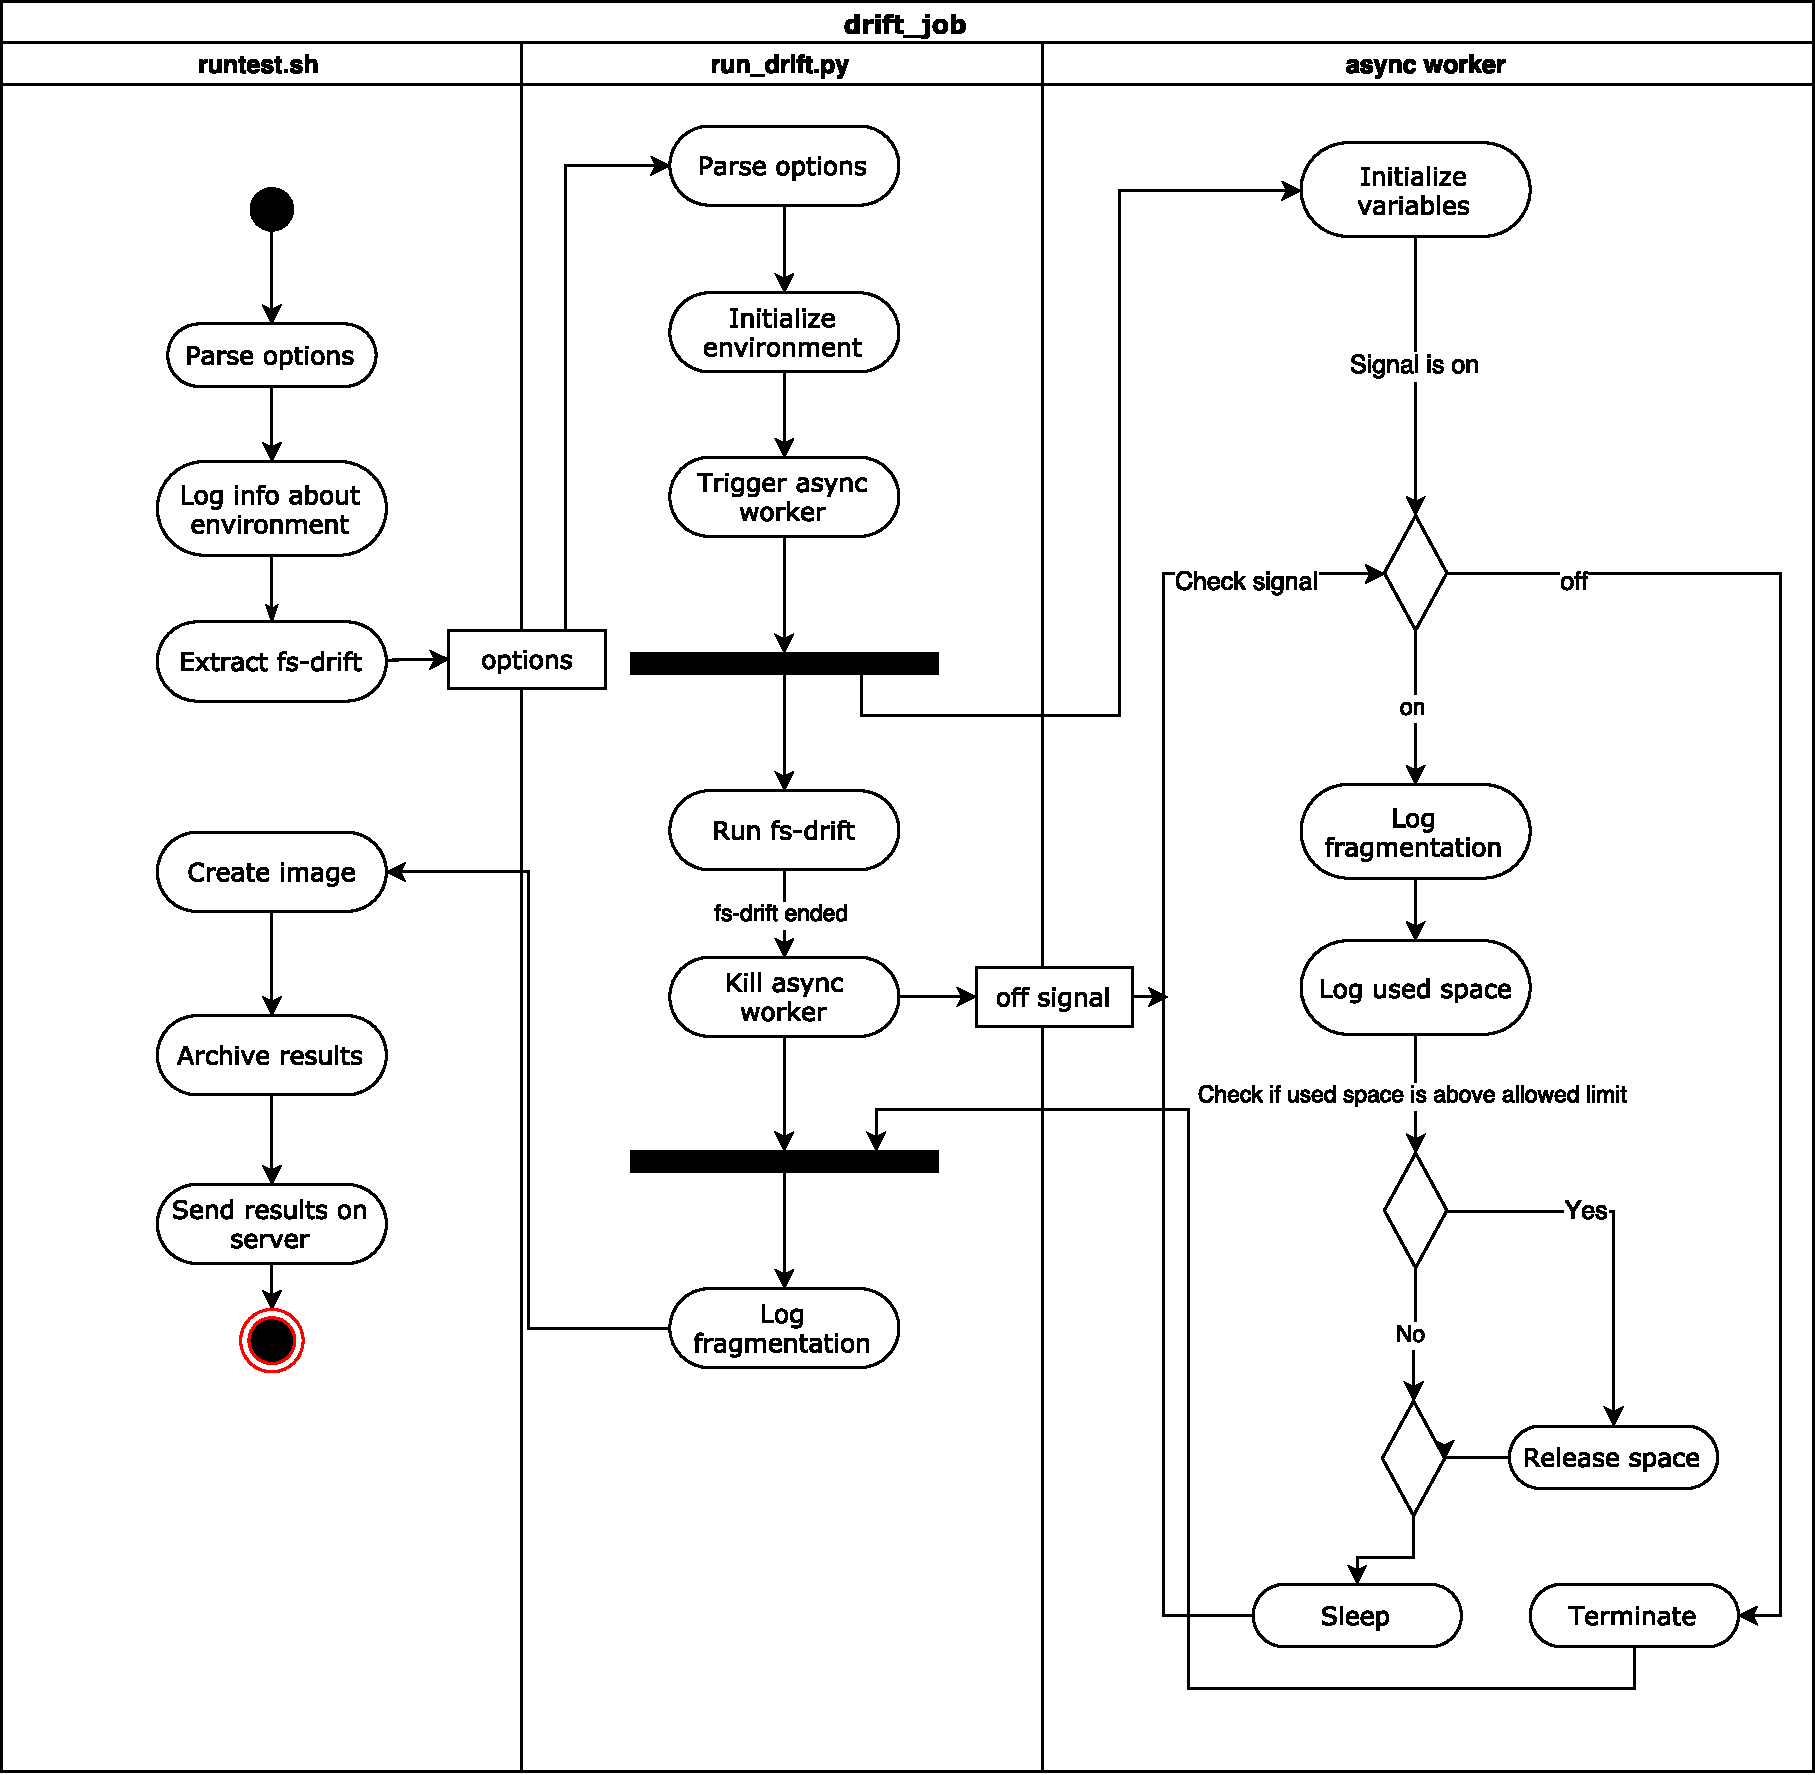
\includegraphics[width=\textwidth,keepaspectratio]{../scripts/drift_job_activity}}
    \caption{Activity diagram of aging test}
    \label{fig:drift_job_activity}
\end{figure}

\chapter{Performance testing of aged file system}
In this chapter, I describe structure of performance test which use images created by previous workflow. In the first section, I present settings of FIO benchmark for the optimal results and in section two, I describe implementation of this test as beaker task.

\section{FIO settings} 

%While designing FIO workload to test performance of aged file system, 

By default, FIO will create one file for every triggered thread. Furtermore, this file is created and opened before FIO begins issuing IO requests. This default settings is unfit for file system aging testing, because the subject of iterest is among others file allocation.

The first step to make FIO workload more relevant to file system aging is to ask for creation of many files for every thread. The number of files was set in such a way, their individual size was approximately $\SI{4}{\kilo\byte}$. FIO will try to open all the files at once, which results in error for more than 102 files, therefore, maximal amount of open files was specified to 100. Furthermore, to include creation of files and allocation into the performance measurement, \texttt{create\_on\_open} was set, so FIO creates file at the moment of opening, if the file does not exist. Another important factor is distribution of which FIO access the files. Default is set to round-robin, but was reset to gauss, so the distribution of file access is more similar to file system aging test.

Similarily to aging test, FIO should perform \texttt{fsync} from time to time. This can be set as amount of write requests after which \texttt{fsync} should be performed.

Overall size is set in such a way, it consumes most of space left after loading the image. Same size is used while testing on fresh file system. Block size is set to $\SI{4}{\kilo\byte}$ as that is default block size of used file systems.

To ensure stable runtime of FIO test, time-based testing is used with runtime of 10 minutes. It is not expected of FIO to issue total specified size, but to measure the performance effectively.


%Volume is randomly removed using random\_delete\_volume.py script. This scriptt globs all files in the filesystem, retrieves information about used volume as well as it's overall size. Then proceeds to randomly choosing files to delete and stops when desired volume is freed. The approach of recursively globbing all files may be inefficient, but this way, we can be sure, that volume is deleted from whole device evenly.

%\section{Inspecting filesystem}

%To determine overall idea about an extent to which is the file system aged, scripts that generate histograms representing fragmentation of used space as well as fragmentation of free space. Both scripts use common linux tools and pyplot to generate the graphics. Both scripts can display linear or logarhytmic Y scale.

%Script extent\_distribution.py makes use of xfs\_io fiemap tool, which is a tool to display extent distribution of a given file and works correctly even for ext* filesystems.

%The script will first recursively crawls the whole filesystem from given top folder and makes a list of all files. Fiemap is then run over every file separately. 

%The only data, that are then parsed from the output, is how many non-contigous extents does the file have. These integers are aggregated to a single list, from which are then counted, and final histogram is made.

%Script free\_space\_fragmentation.py use the tool e2freefrag, which runs over a device, and outputs the histogram of free space fragmentation in texutal form. Script will store this output and then easily parse the histogram and aggregate the data into a graphic form.

\section{Test structure}
Performance testing of created images is contained in Beaker task recipe\_fio\_aging. Upon instalation of necessary tools (libs, fio), the package finds and downloads coresponding file system image according to obtained parameters. As shown, images are stored compressed, therefore decompression is needed after download. Once these steps are succesfully completed, testing phase can begin.

Before every test, initialization is performed by running \texttt{sync}, \texttt{fstrim} and dropping caches.

At first, performance measurements of fresh file system is done. Test configuration of fresh and aged test is similar, with an exception, that after testing fresh file system, FIO will delete all the created files. This is disabled for aged tests, because post-test fragmentation is gathered afterwards.

After testing fresh file system, image is loaded and mouted. If the mounted file system utilize too much space, some files can be randomly deleted. Afterwards, pre-test fragmentation is logged and environment is initalized. When the test is over, post-test fragmentation is gathered.

For statistical correctness, these tests can run in loops $n$ times. Fresh and aged testing is divided into separate loops.

After last iteration, the results are archived and sent to data-collecting server. 

For better oversight of the tests functionality, its activity diagram is presented as Figure~\ref{fig:rec_activity}

Parameters available for recipe\_fio\_aging:
\begin{compactenum}
  \item sync, flag to signalise wheather or not to send data to server (usefull for developing purposes)
  \item numjobs, number of test repetitions. For statistical stability
  \item mountpoint
  \item device
  \item recipe, parameters to pass to FIO test
  \item tag, string to distinguish different tests
  \end{compactenum}

\begin{figure}[ht]
    \centering
    \fbox{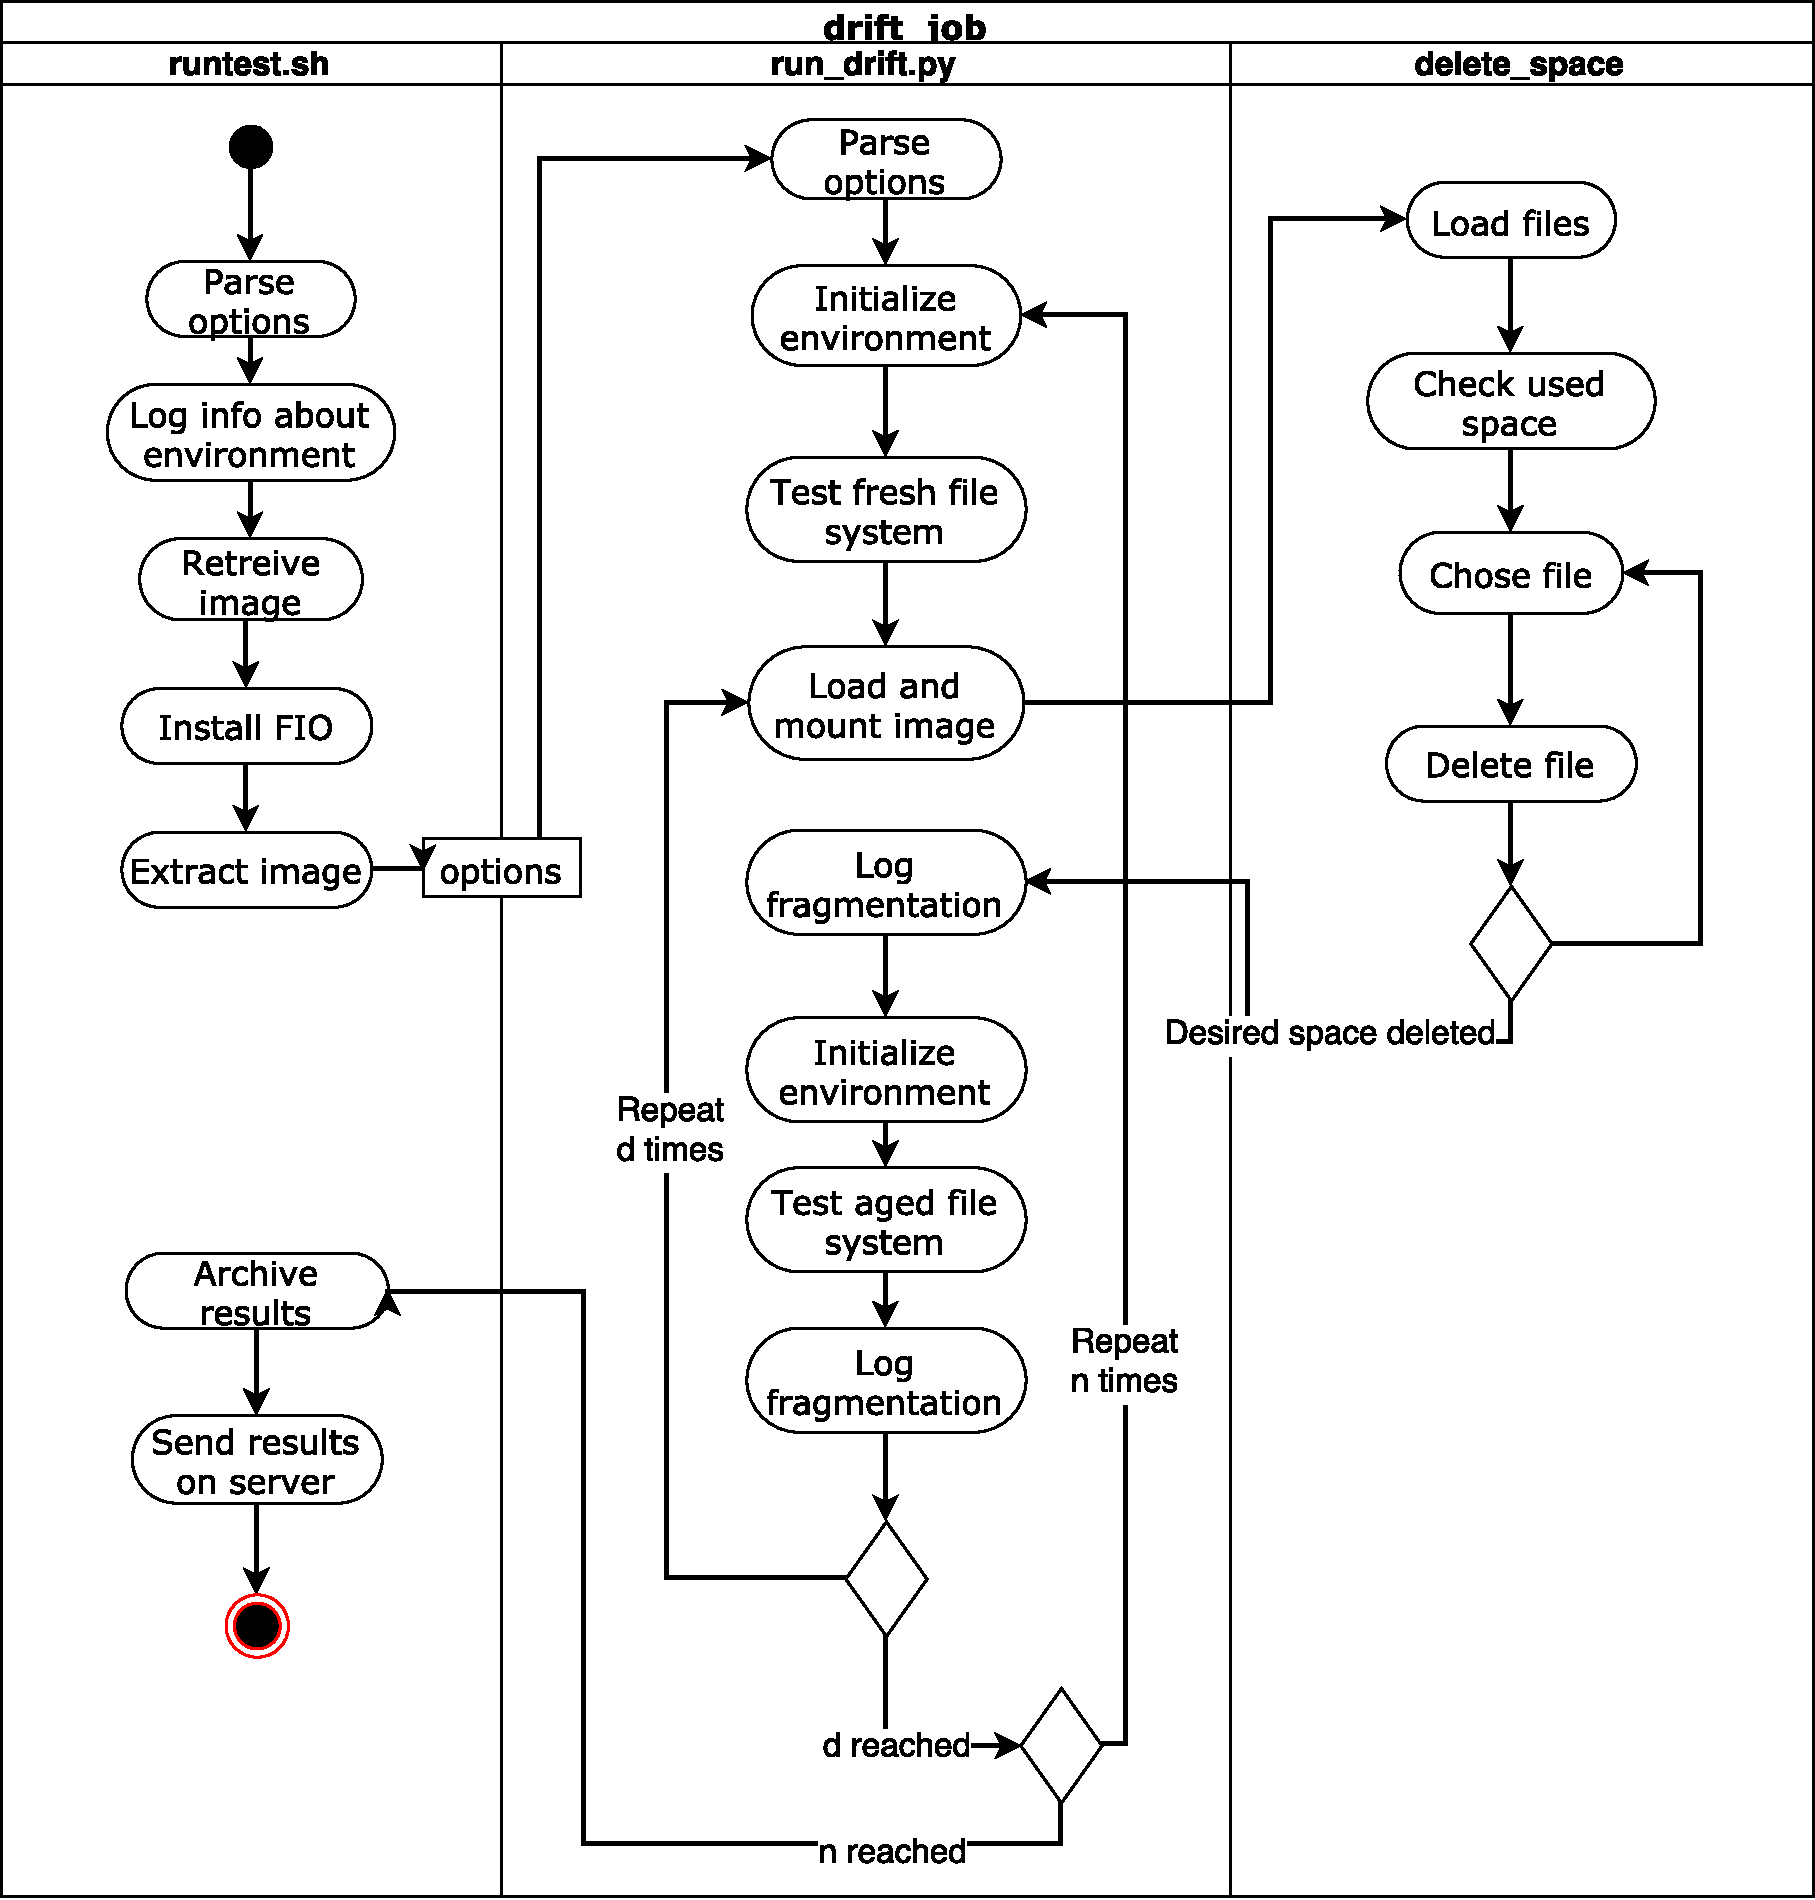
\includegraphics[width=\textwidth,keepaspectratio]{../scripts/recipe_fio_aging_activity}}
    \caption{Activity diagram of testing of aged file system}
    \label{fig:rec_activity}
\end{figure}







\chapter{Results}
This chapter present results of implemented tests. In the first section I describe environment used for testing. In the second section, I describe means of data evaluation. In the third section, I show elementary differences between fresh and aged file systems. In the fourth section, I describe differences between two tested file systems (XFS, Ext4) in terms of aging. In fifth section I demonstrate the effect file system aging have on underlying storage.

\section{Testing environment}
In this section, I describe testing environment and storage used for testing with created tests. The testing machines were available to me from a pool of systems of Red Hat Beaker environment.

\begin{tabular}{|l|l|}
\hline
   \multicolumn{2}{|l|}{Machine\,1} \\ \hline
    Model & Lenovo\texttrademark System x3250\,M6 \\
    \hline
    Processor & Intel\textsuperscript\textregistered Xeon\textsuperscript\textregistered E3-1230\,v5 \\
    \hline
    Clock speed & $\SI{3.40}{\giga\hertz}$ (4 cores) \\
    \hline
    Memory & $\SI{1628}{\mega\byte}$ \\
    \hline
    \multicolumn{2}{|l|}{Storage} \\ \hline
    Device & HP Proliant HardDrive\\ \hline
    Interface & SAS\\ \hline
    Capacity & $\SI{600}{\giga\byte}$\\ \hline
\hline
   \multicolumn{2}{|l|}{Machine\,2} \\ \hline
    Model & Lenovo\texttrademark System x3250\,M6 \\
    \hline
    Processor & Intel\textsuperscript\textregistered Xeon\textsuperscript\textregistered E3-1230\,v5 \\
    \hline
    Clock speed & $\SI{3.40}{\giga\hertz}$ (4 cores) \\
    \hline
    Memory & $\SI{1628}{\mega\byte}$ \\
    \hline
    \multicolumn{2}{|l|}{Storage} \\ \hline
    Device\,1 & HP Proliant HardDrive \\ \hline
    Interface & SAS\\ \hline
    Capacity & $\SI{600}{\giga\byte}$\\ \hline
    Device\,2 & SSD \\ \hline
    Interface & SATA\\ \hline
    Capacity & $\SI{120}{\giga\byte}$\\ \hline
\hline
   \multicolumn{2}{|l|}{Machine\,3} \\ \hline
    Model & IBM x3650 System\,M4 \\
    \hline
    Processor & Intel\textsuperscript\textregistered Xeon\textsuperscript\textregistered E5-2620\,v2 \\
    \hline
    Clock speed & $\SI{2.10}{\giga\hertz}$  (4 cores) \\
    \hline
    Memory &  $\SI{65536}{\mega\byte}$\\
    \hline
    \multicolumn{2}{|l|}{Storage} \\ \hline
    Device\,1\&2 & IBM Solid State Drive\\ \hline
    Interface &  SATA\\ \hline
    Capacity & $\SI{400}{\giga\byte}$\\ \hline
\end{tabular}

\section{Data processing}
Accounting for great amount of data generated by the tests, some kind of automatic processing needs to be implemented to make evaluation easier for humans. Therefore, I developed set of scripts which can compare results of two different runs of implemented test. The output of those script is human-readable HTML report. The report displays information about testing environment and different charts described bellow. All the reports generated from the tests can be found in Appendix A. The scripts used to generate reports are part of this thesis in form of electronic appendix

\subsection{Fragmentation}
During the tests, two types of fragmentation were recorded, namely fragmentation of used space and fragmentation of free space.

To find out fragmentation of used space, \texttt{xfs\_io fiemap} was used. This tool can display physical mapping of any file, using $\SI{512}{\byte}$ blocks. Therefore, if run on every file in file system, histogram of fragments of used space can be computed.

Generally, fragmentation of free space is easier to obtain, since this information is stored in the metadata of file system. However, the way of reading the information differs through implementations of file systems. In Ext4, the tool \texttt{e2freefrag} displays histogram of free space of Ext* file system. When looking for this information in XFS, at~first user has to find number of allocation grups in the file system instance. Then, for every allocation group, histogram of free space can be obtained using \texttt{xfs\_db}.

As stated, in the aging test, fragmentation of free space is logged periodically, allowing for an analysis of how fragmentation evolves in time. For the purpose of visualising this evolution, 3D charts are introduced in the final reports.

\subsection{Fs-drift}
The main researched output of fs-drift is an \emph{evolution} of latency of different operations. This property is displayed as a chart with elapsed time on X axis and measured latency on Y axis. Since the data are quite noisy, interpolation and filtering using Savitzky-Golay filter had to be used for meaningfull display of latency change in time. Additionally linear regression is computed and displayed for every operation providing even more insight into the effects of aging through test.

\subsection{FIO}
The output of FIO is recorded bandwidth and latency through tests. Since topic of research when using FIO was \emph{state} of file system in terms of performance, statistics are computed from the whole test run. These statistics are minimum and maximum value, first and second quartile and median. These atributes are then displayed on a chart in form of boxplot. Latency and bandwidth have separate charts. On the X axis, state of file system utilization is displayed and on the Y axis there is throughput or latency.

\section{Performance of aged file system}
The file sysem aging tool succesfully induced fragmentation on all used devices. From the results generated by aging tool, it is apparent, that the aging process negatively affects performance of file systems. Figure shows evolution of free space fragmetation when using XFS file system on signle SAS HDD. Figure X shows 


\section{Differences betweem XFS and EXT4}


\section{Differences amoung storage devices}











\chapter{Conclusion}


\printbibliography

\appendix %% Start the appendices.
\chapter{Reports}
\chapter{Examples}
\lstset{language=XML, 
numbers=left, 
frame=single, 
commentstyle=\color{dkgreen}, 
basicstyle={\scriptsize\ttfamily}, 
keywordstyle=\color{blue}, 
%identifierstyle=\color{blue}, 
stringstyle=\color{red},
captionpos=t,
showstringspaces=false,
breaklines=true,
breakatwhitespace=false,
tabsize=3,
caption={},
}


\begin{lstlisting}[language=xml, caption={Specifying OS to be installed}][frame=single]
<distroRequires>
  <and>
    <distro_family op="=" value="RedHatEnterpriseLinux7"/>
    <distro_variant op="=" value="Server"/>
    <distro_name op="=" value="RHEL-7.3"/>
    <distro_arch op="=" value="x86_64"/>
  </and>
</distroRequires>
\end{lstlisting}

\begin{lstlisting}[language=xml, caption={Configuring environment using kickstart}][frame=single]
<kickstart>
  <![CDATA[
    install
    lang en_US.UTF-8
    skipx
    keyboard us
    rootpw redhat
    firewall --disabled
    authconfig --enableshadow --enablemd5
    selinux --enforcing
    timezone --utc Europe/Prague

    bootloader --location=mbr --driveorder=sda
    zerombr
    clearpart --all --initlabel --drives=sda
    part /boot --fstype=ext2 --size=200 --asprimary --label=BOOT --ondisk=sda
    part /mnt/tests --fstype=ext4 --size=40960 --asprimary --label=MNT --ondisk=sda
    part / --fstype=ext4 --size=1 --grow --asprimary --label=ROOT  --ondisk=sda
    reboot
    %packages --excludedocs --ignoremissing --nobase
    @core
    wget
    python
    dhcpv6-client
    dhclient
    yum
]]>
</kickstart>
\end{lstlisting}

\begin{lstlisting}[language=xml, caption={Executing task and passing arguments}][frame=single]
      <task name="/kernel_fsperf/storage_generator" role="STANDALONE">
        <params>
          <param name="TEST_PARAM_STORAGE_GENERATOR" value="-s create -f ext4 -t single -m /RHTSspareLUN1 -d /dev/sdc -T 1SASHDD_ext4"/>
        </params>
      </task>
\end{lstlisting}

\begin{lstlisting}[language=xml, caption={Configuring storage using storage generator in beaker environment}][frame=single]
      <task name="/kernel_fsperf/storage_generator" role="STANDALONE">
        <params>
          <param name="TEST_PARAM_STORAGE_GENERATOR" value="-s create -f xfs -t lvm -m /RHTSspareLUN1 -r jokerlvm -T 2SATASSDLVM_xfs"/>
        </params>
      </task>
\end{lstlisting}

\end{document}

